\section{Observation}
\label{observation}
\label{sec:Observation}

To systematically expose this attack surface, we ask five questions:
\begin{packeditemize}
    \item \textbf{Q1:} In an open-vocabulary autoregressive system, what is the effective emotion decision interface?
    \item \textbf{Q2:} Is perceived emotion merely reported, or does it function as a behavior-control variable for generation?
    \item \textbf{Q3:} Why do classifier-style SER attacks fail even under stronger perturbation budgets?
    \item \textbf{Q4:} Across heterogeneous Audio LLMs, what part of the emotion mechanism is shared, and what part is model-specific?
    \item \textbf{Q5:} If emotion is verbalized as a token, where is the controllable boundary along model depth?
\end{packeditemize}

We answer these questions through five observations.

\subsection{Empirical Findings}
\label{sec:obs_empirical_findings}
\label{sec:obs-allm-universal}
\label{sec:clean-emotion-observation}

% =========================================================
% Observation 1
% =========================================================

\subsubsection{The Effective Emotion Decision Interface is a Compact Subspace}
\label{sec:obs_q1}

To resolve Q1, we first inspect how an Audio LLM verbalizes emotion at the first decoding step.
Unlike conventional speech emotion recognition (SER) models, Audio LLMs do not expose an explicit classification head for emotion prediction.
Instead, they express emotion through autoregressive decoding over a large vocabulary, which raises a basic question: is emotion determined over the full vocabulary space, or does a smaller implicit decision interface exist?

\begin{figure}[!t]
    \centering
    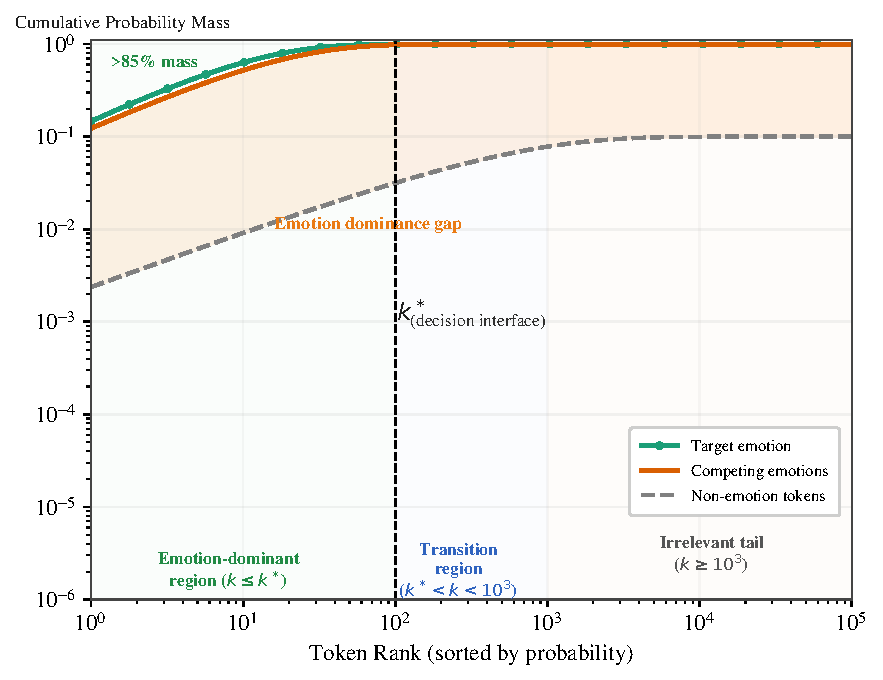
\includegraphics[width=\linewidth]{figure/probability_mass_emotion_tokens.pdf}
    \caption{
    \textbf{Concentration of probability mass on emotion tokens.}
    The cumulative next-token probability mass rapidly saturates within a small set of top-ranked tokens.
    Emotion-related tokens dominate this region, while non-emotion tokens contribute negligibly.
    }
    \label{fig:fig2}
\end{figure}

As shown in Figure~\ref{fig:fig2}, the cumulative next-token probability mass rapidly concentrates within the top-ranked tokens.
More importantly, this high-mass region is dominated by emotion-related tokens, while non-emotion tokens contribute only marginally.
We observe a clear cutoff point $k^*$, beyond which additional tokens add negligible probability mass.
This indicates that emotion prediction is not performed over the full vocabulary simplex.
Rather, the model implicitly restricts its decision to a compact subset of candidate tokens, within which emotion-related tokens compete for dominance.
From this, we derive the first observation as follows.

\begin{obsbox}
\textbf{Observation 1 (Decision interface).}
Emotion prediction in Audio LLMs is governed by a compact top-$k$ token region, forming an implicit decision interface rather than a full-vocabulary decision.
\end{obsbox}

% =========================================================
% Observation 2
% =========================================================

\subsubsection{Perceived Emotion Acts as a Behavior-Control Variable}
\label{sec:obs_q2}

To address Q2, we next examine whether emotion in Audio LLMs is simply reported as an output label, or whether it functions as an internal control variable that shapes generation behavior.
This distinction is critical: an attack on emotion is only meaningful if it can alter \emph{what the model says}, rather than just \emph{how the model labels the input}.

\begin{figure}[!t]
    \centering
    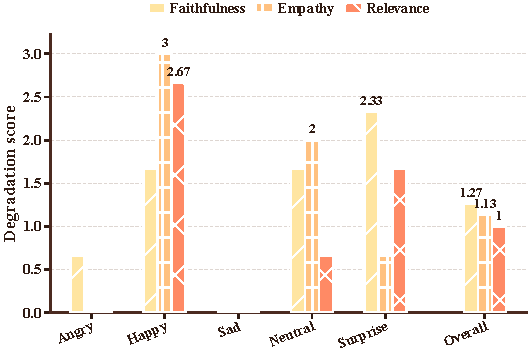
\includegraphics[width=\linewidth]{figure/fig_table1_response_quality_bars.pdf}
    \caption{
    \textbf{Response degradation under emotion misperception.}
    We measure degradation as $\Delta=\text{Aligned}-\text{Conflict}$ on Faithfulness, Empathy, and Relevance.
    Larger $\Delta$ indicates greater response degradation under conflicting perceived emotion.
    }
    \label{fig:q2_bar}
\end{figure}

\begin{figure*}[!t]
    \centering
    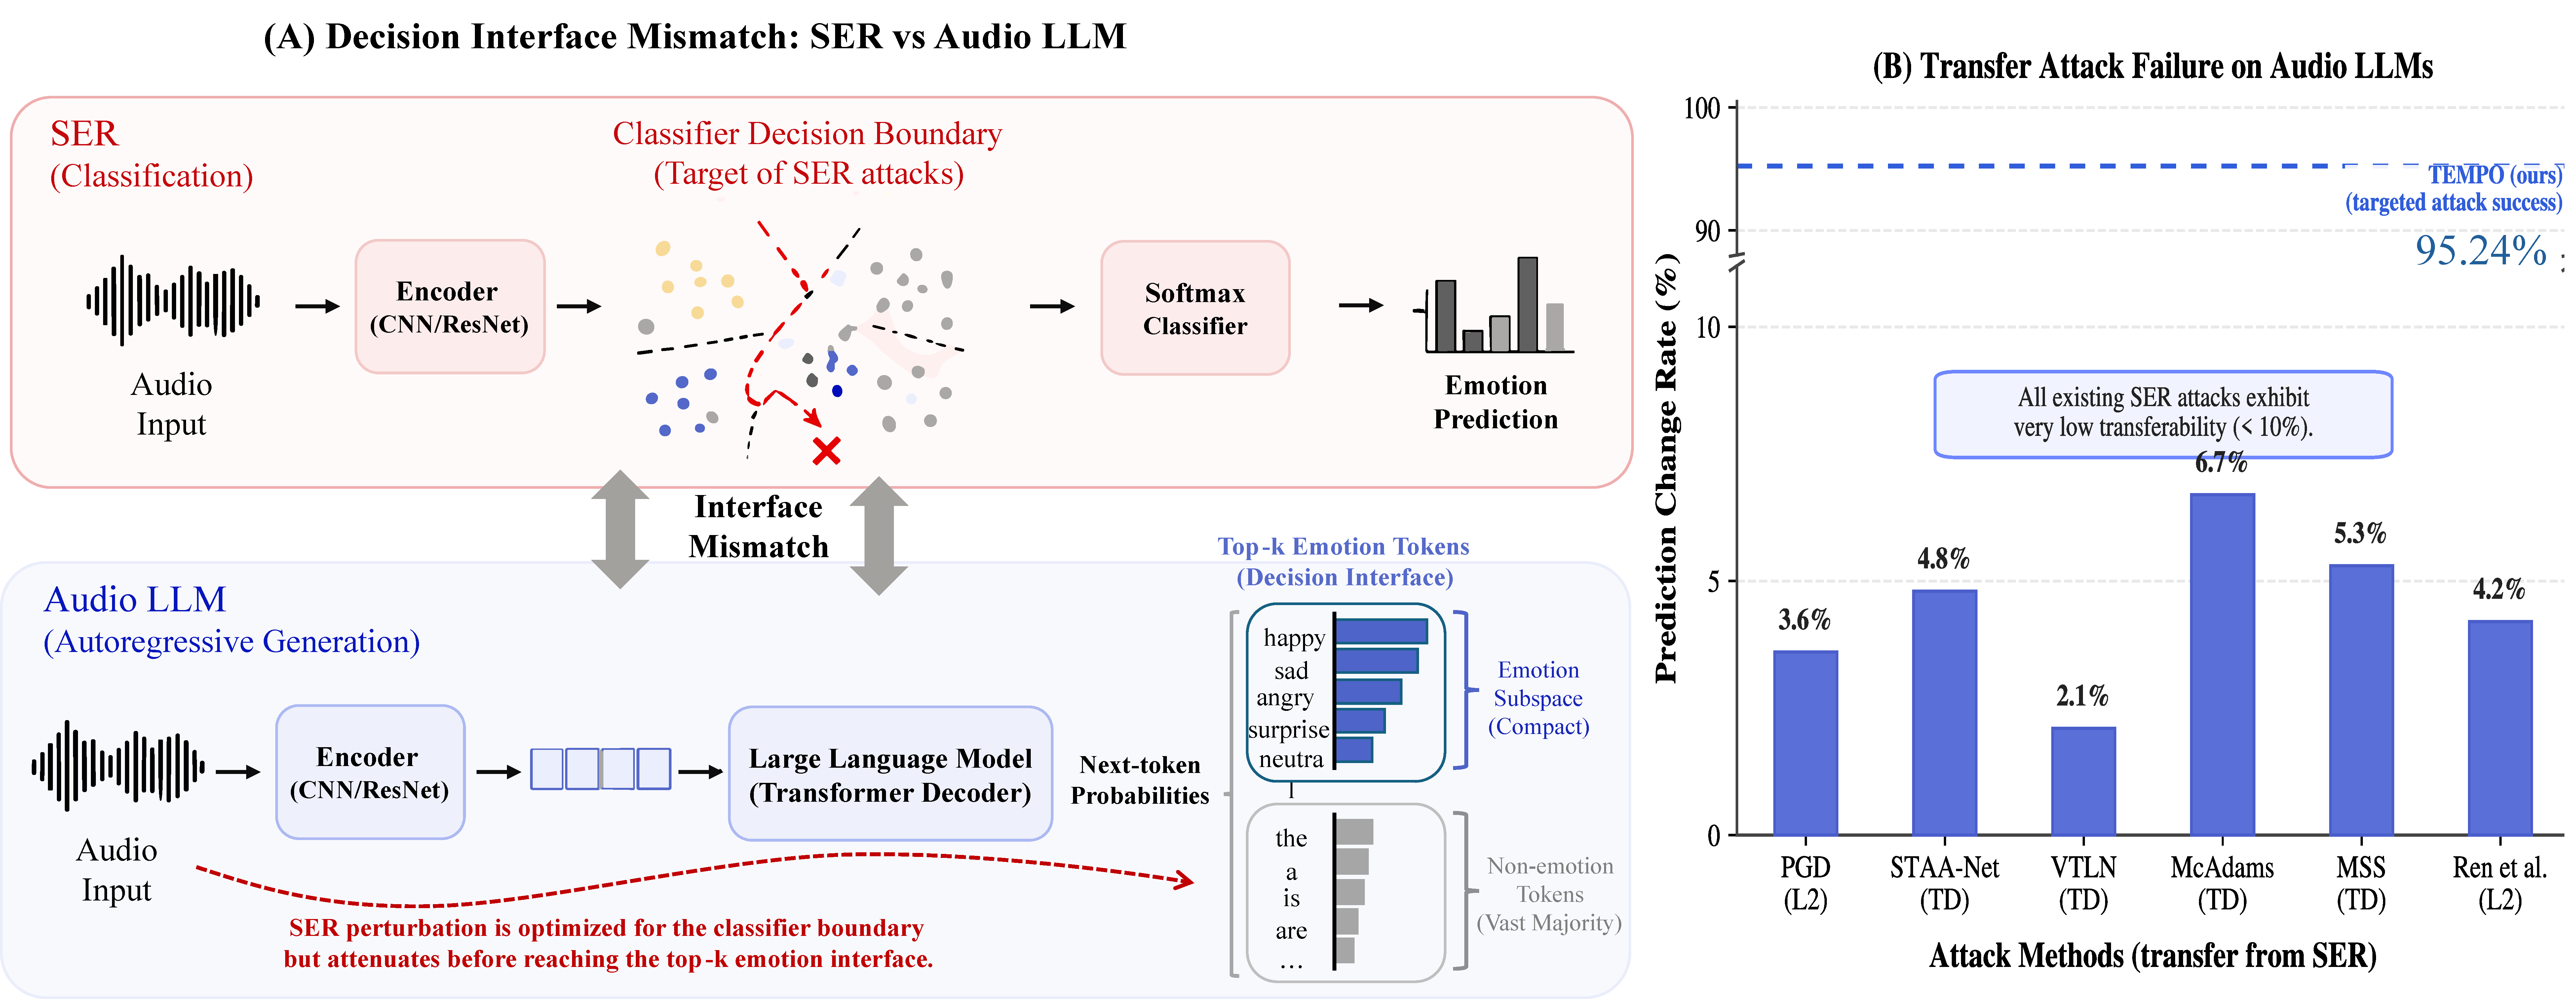
\includegraphics[width=0.95\textwidth]{figure/fig_obs3_interface_mismatch.pdf}
    \caption{
    \textbf{Failure of SER attacks due to decision interface mismatch.}
    \textbf{(A)} SER attacks are optimized to cross classifier decision boundaries, while Audio LLMs determine emotion through a compact top-$k$ token interface during autoregressive decoding.
    This mismatch prevents perturbations from reaching the actual decision interface.
    \textbf{(B)} As a result, all existing SER attacks exhibit low transferability (typically $<10\%$ prediction change rate) on Audio LLMs, despite strong performance on surrogate SER models.
    }
    \label{fig:obs3}
\end{figure*}

To isolate this effect, we construct an aligned-versus-conflict evaluation protocol.
For each audio input, the model is prompted under two conditions: an \emph{Aligned} condition, where the perceived emotion matches the ground truth, and a \emph{Conflict} condition, where the perceived emotion is replaced with a contrasting affective description while keeping the semantic content unchanged.
As shown in Figure~\ref{fig:q2_bar}, the resulting degradation is both significant and highly structured.
In particular, \textit{happy} inputs exhibit the largest degradation, with $\Delta_{\text{Empathy}} = +3.00$ and $\Delta_{\text{Relevance}} = +2.50$, while \textit{neutral} and \textit{sad} inputs show near-zero change across all metrics.

This non-uniform pattern indicates that the impact of emotion is not incidental.
Instead, the perceived affect systematically modulates the model's response behavior.
Beyond aggregate scores, we also observe qualitative shifts in generation.
For example, when a neutral factual statement such as \textit{``The package is scheduled to arrive tomorrow afternoon''} is interpreted under a conflicting emotional condition, the model introduces affective content (e.g., frustration or concern) that is not grounded in the input.
Thus, changing the perceived emotion does not merely alter the label; it shifts response style, tone, and content selection.
We summarize this finding as follows.

\begin{obsbox}
\textbf{Observation 2.} Perceived emotion is not merely reported, but acts as a latent control variable that causally shapes downstream generation behavior.
\end{obsbox}

% =========================================================
% Observation 3
% =========================================================

\subsubsection{Conventional SER Attacks Fail Due to Decision Interface Mismatch}
\label{sec:obs_q3}

To answer Q3, we examine whether existing adversarial attacks developed for speech emotion recognition (SER) models can be directly applied to Audio LLMs.
Since both tasks involve emotion understanding from audio, one might expect such attacks to transfer.

We evaluate six representative SER adversarial attacks, including PGD, STAA-Net, VTLN, McAdams, MSS, and Ren et al., by directly transferring them to Audio LLMs.
As shown in Figure~\ref{fig:obs3}(B), all methods exhibit consistently low prediction change rates, typically below $10\%$, even when using untargeted objectives and significantly larger perturbation budgets.
This indicates that conventional SER attacks fail to effectively manipulate emotion predictions in Audio LLMs.

The failure is not merely due to insufficient attack strength, but reflects a mismatch in the decision interface.
Conventional SER models rely on a fixed classifier decision boundary, where adversarial perturbations are designed to shift representations across this boundary.
In contrast, as shown in Observation~1, Audio LLMs determine emotion through autoregressive decoding, where the effective decision interface is a compact top-$k$ token subspace.
As illustrated in Figure~\ref{fig:obs3}(A), perturbations optimized for classifier boundaries do not reliably reach or influence this token-level interface.
Instead, they are attenuated or become irrelevant before affecting the model's internal emotion competition.
This explains why increasing perturbation magnitude does not significantly improve transferability: the attack is targeting the wrong interface.
From this, we derive the following observation.

\begin{obsbox}
\textbf{Observation 3.}
Conventional SER adversarial attacks fail to transfer to Audio LLMs because they optimize a mismatched decision interface—classifier-level boundaries rather than the autoregressive top-$k$ emotion interface used by the model.
\end{obsbox}



\subsubsection{Competitive Structure is Shared Across Models}
\label{sec:obs_q4}

For Q4, we further investigate whether the compact token-level interface exhibits consistent structure across different Audio LLMs.

\begin{figure}[!t]
    \centering
    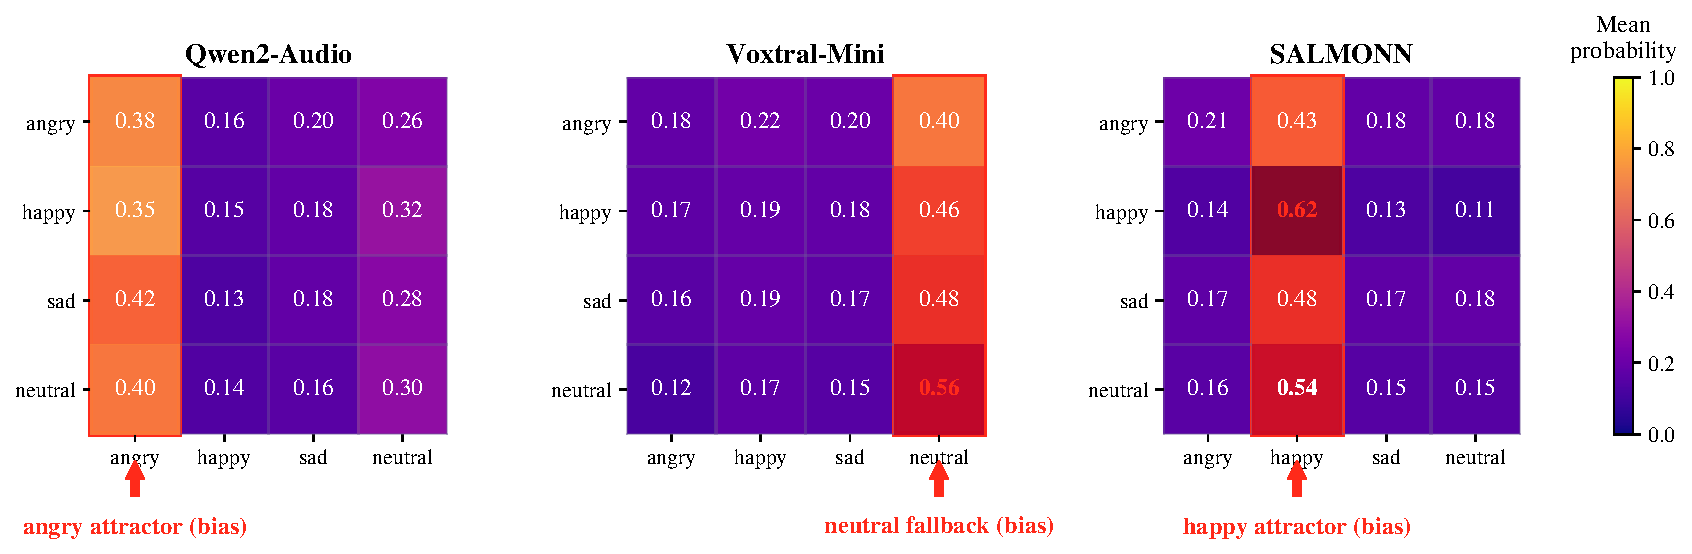
\includegraphics[width=\linewidth]{figure/fig_final_competition_heatmaps.pdf}
    \caption{
    \textbf{Cross-model emotion competition fields.}
    All models exhibit soft competition among candidate emotions, but their dominant bias centers differ:
    Qwen2-Audio tends toward \textit{angry}, Voxtral-Mini falls back to \textit{neutral}, 
    and SALMONN is attracted to \textit{happy}.
    }
    \label{fig:obs4_competition}
\end{figure}

One possible hypothesis is that different models share a common emotion attractor, where each emotion consistently dominates across architectures.
However, Figure~\ref{fig:obs4_competition} shows that this hypothesis does not hold.
The dominant preference varies significantly across models: Qwen2-Audio leaks probability mass toward \textit{angry}, Voxtral-Mini exhibits a \textit{neutral} fallback, and SALMONN shows a \textit{happy} attractor.
Despite this variation, a consistent structural pattern emerges.
Across all models, emotion prediction is not performed independently for each label, but is organized as soft competition among a compact set of candidate emotions.
Therefore, the shared property is not a universal attractor, but a competitive decision structure.

\begin{obsbox}
\textbf{Observation 4 (Competitive structure).}
Emotion prediction does not share a universal attractor across models, but consistently exhibits a compact competitive structure over candidate emotions.
\end{obsbox}

\subsubsection{The Control Bottleneck Emerges at Intermediate Layers}
\label{sec:obs_q5}

Finally, to address Q5, we investigate where the competitive emotion structure becomes controllable within the model.

\begin{figure}[!t]
    \centering
    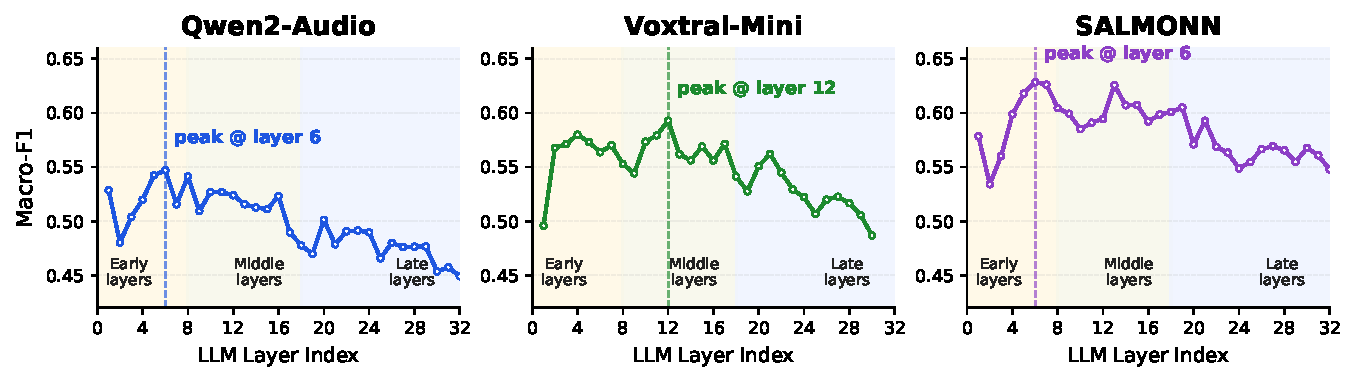
\includegraphics[width=\linewidth]{figure/fig_final_midlayer_peaks.pdf}
    \caption{
    \textbf{Layer-wise emotion separability.}
    Emotion probing performance peaks at intermediate layers across all models,
    indicating that the effective control boundary emerges before decoding.
    }
    \label{fig:obs5_layer}
\end{figure}

If emotion is ultimately expressed as an output token, one might expect the final layer to provide the strongest separability.
However, Figure~\ref{fig:obs5_layer} shows the opposite trend.
Across all models, emotion separability peaks at intermediate layers rather than the final layer: Qwen2-Audio and SALMONN peak around layer 6, while Voxtral-Mini peaks around layer 12.
This indicates that emotion is internally organized before the decoding stage.
The final layer emits the decision, but does not define the decision boundary.
This leads to the final observation.

\begin{obsbox}
\textbf{Observation 5 (Control bottleneck).}
The steerable emotion boundary emerges at intermediate layers before decoding, 
providing a natural control interface for layer-adaptive manipulation.
\end{obsbox}
